\documentclass[a4paper, 12pt]{article}
\usepackage[T2A]{ fontenc }
\usepackage[utf8]{ inputenc }
\usepackage[english, russian]{babel}
\usepackage{amsmath,amsfonts,amssymb,amsthm,mathtools}
\usepackage[colorlinks, linkcolor = blue]{hyperref}
\usepackage{upgreek}
\usepackage[left = 2cm, right = 2cm, top = 2cm, bottom = 3cm, bindingoffset = 0cm]{geometry}
\usepackage{graphicx}
\usepackage{multirow}
\usepackage{xcolor}
\usepackage{tabularx}
\title{ Differenciator }
\author{Valiev Ruzal}
\date{December 2023}
\begin{document}
\maketitle
\section{Expression}
Taking this fact into account...\newline
$ sin( x )  +  cos(  { x } ^ {\small 2 }  ) $\newline
It is known that...\newline
$ cos( x )  + -1 \cdot  sin(  { x } ^ {\small 2 }  )  \cdot 2 \cdot x$\newline
We'll determine the domain and range of the function.\newline
$ sin( x )  +  cos(  { x } ^ {\small 2 }  ) $\newline
Let's examine the case when the variables are independent.\newline
$ cos( x )  + -1 \cdot  sin(  { x } ^ {\small 2 }  )  \cdot 2 \cdot x$\newline
Let's assume our statement is false, then...\newline
$ cos( x )  + -1 \cdot  sin(  { x } ^ {\small 2 }  )  \cdot 2 \cdot x$\newline
Let's imagine that...\newline
$-1 \cdot  sin( x )  + -1 \cdot  cos(  { x } ^ {\small 2 }  )  \cdot 2 \cdot x \cdot 2 \cdot x + -1 \cdot  sin(  { x } ^ {\small 2 }  )  \cdot 2$\newline
Using the concept of symmetry...\newline
$ sin( x )  +  cos(  { x } ^ {\small 2 }  ) $\newline
Let's investigate the convergence/divergence of this series.\newline
$ cos( x )  + -1 \cdot  sin(  { x } ^ {\small 2 }  )  \cdot 2 \cdot x$\newline
It should be noted that\newline
$ cos( x )  + -1 \cdot  sin(  { x } ^ {\small 2 }  )  \cdot 2 \cdot x$\newline
Suppose that...\newline
$-1 \cdot  sin( x )  + -1 \cdot  cos(  { x } ^ {\small 2 }  )  \cdot 2 \cdot x \cdot 2 \cdot x + -1 \cdot  sin(  { x } ^ {\small 2 }  )  \cdot 2$\newline
We'll establish a correspondence between...\newline
$-1 \cdot  sin( x )  + -1 \cdot  cos(  { x } ^ {\small 2 }  )  \cdot 2 \cdot x \cdot 2 \cdot x + -1 \cdot  sin(  { x } ^ {\small 2 }  )  \cdot 2$\newline
Let's reason logically: if... then...\newline
$-1 \cdot  cos( x )  + -1 \cdot  ( -1 \cdot  sin(  { x } ^ {\small 2 }  )  \cdot 2 \cdot x \cdot 2 \cdot x +  cos(  { x } ^ {\small 2 }  )  \cdot 2 )  \cdot 2 \cdot x + -1 \cdot  cos(  { x } ^ {\small 2 }  )  \cdot 2 \cdot x \cdot 2 + -1 \cdot  cos(  { x } ^ {\small 2 }  )  \cdot 2 \cdot x \cdot 2$\newline
It's essential to consider the implications of this axiom.\newline
$ sin( x )  +  cos(  { x } ^ {\small 2 }  ) $\newline
We'll simplify the expression by factoring.\newline
$ cos( x )  + -1 \cdot  sin(  { x } ^ {\small 2 }  )  \cdot 2 \cdot x$\newline
Let's consider the case when\newline
$ cos( x )  + -1 \cdot  sin(  { x } ^ {\small 2 }  )  \cdot 2 \cdot x$\newline
Taking this fact into account...\newline
$-1 \cdot  sin( x )  + -1 \cdot  cos(  { x } ^ {\small 2 }  )  \cdot 2 \cdot x \cdot 2 \cdot x + -1 \cdot  sin(  { x } ^ {\small 2 }  )  \cdot 2$\newline
Let's reason logically: if... then...\newline
$-1 \cdot  sin( x )  + -1 \cdot  cos(  { x } ^ {\small 2 }  )  \cdot 2 \cdot x \cdot 2 \cdot x + -1 \cdot  sin(  { x } ^ {\small 2 }  )  \cdot 2$\newline
It is known that...\newline
$-1 \cdot  cos( x )  + -1 \cdot  ( -1 \cdot  sin(  { x } ^ {\small 2 }  )  \cdot 2 \cdot x \cdot 2 \cdot x +  cos(  { x } ^ {\small 2 }  )  \cdot 2 )  \cdot 2 \cdot x + -1 \cdot  cos(  { x } ^ {\small 2 }  )  \cdot 2 \cdot x \cdot 2 + -1 \cdot  cos(  { x } ^ {\small 2 }  )  \cdot 2 \cdot x \cdot 2$\newline
We'll simplify the expression by factoring.\newline
$-1 \cdot  cos( x )  + -1 \cdot  ( -1 \cdot  sin(  { x } ^ {\small 2 }  )  \cdot 2 \cdot x \cdot 2 \cdot x +  cos(  { x } ^ {\small 2 }  )  \cdot 2 )  \cdot 2 \cdot x + -1 \cdot  cos(  { x } ^ {\small 2 }  )  \cdot 2 \cdot x \cdot 2 + -1 \cdot  cos(  { x } ^ {\small 2 }  )  \cdot 2 \cdot x \cdot 2$\newline
Let's consider the case when\newline
$-1 \cdot -1 \cdot  sin( x )  + -1 \cdot  (  ( -1 \cdot  cos(  { x } ^ {\small 2 }  )  \cdot 2 \cdot x \cdot 2 \cdot x + -1 \cdot  sin(  { x } ^ {\small 2 }  )  \cdot 2 )  \cdot 2 \cdot x + -1 \cdot  sin(  { x } ^ {\small 2 }  )  \cdot 2 \cdot x \cdot 2 + -1 \cdot  sin(  { x } ^ {\small 2 }  )  \cdot 2 \cdot x \cdot 2 )  \cdot 2 \cdot x + -1 \cdot  ( -1 \cdot  sin(  { x } ^ {\small 2 }  )  \cdot 2 \cdot x \cdot 2 \cdot x +  cos(  { x } ^ {\small 2 }  )  \cdot 2 )  \cdot 2 + -1 \cdot  ( -1 \cdot  sin(  { x } ^ {\small 2 }  )  \cdot 2 \cdot x \cdot 2 \cdot x +  cos(  { x } ^ {\small 2 }  )  \cdot 2 )  \cdot 2 + -1 \cdot  ( -1 \cdot  sin(  { x } ^ {\small 2 }  )  \cdot 2 \cdot x \cdot 2 \cdot x +  cos(  { x } ^ {\small 2 }  )  \cdot 2 )  \cdot 2$\newline
\newpage
\begin{figure} [!ht]
\begin{flushleft}
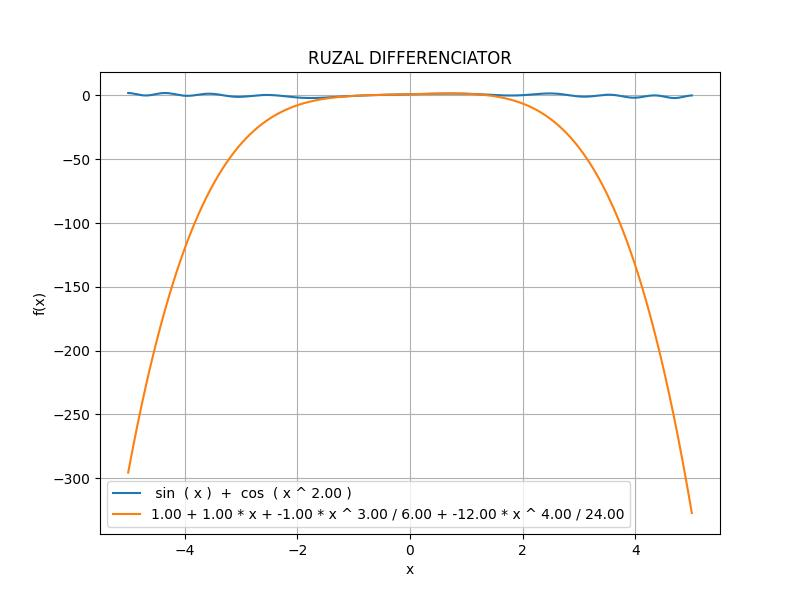
\includegraphics[scale = 0.700000]{taylor.jpeg}
\end{flushleft}
\end{figure}
Taking this fact into account...\newline
$ sin( x )  +  cos(  { x } ^ {\small 2 }  ) $\newline
Considering the behavior of the function at critical points.\newline
$ cos( x )  + -1 \cdot  sin(  { x } ^ {\small 2 }  )  \cdot 2 \cdot x$\newline
\newpage
\begin{figure} [!ht]
\begin{flushleft}
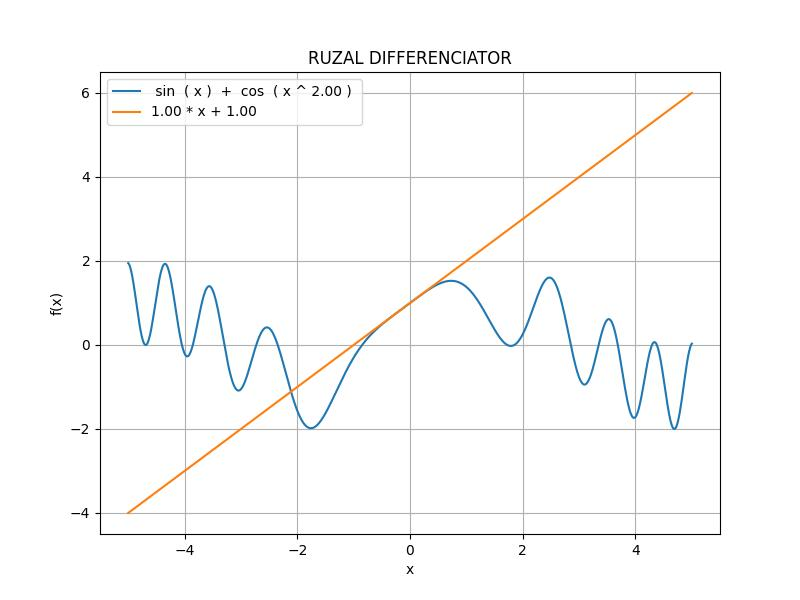
\includegraphics[scale = 0.700000]{tangent.jpeg}
\end{flushleft}
\end{figure}
\end{document}